\section{What the step should depend on: the anchor's reliability relative to the trained branch}\label{sec:finding3}

Sections~\ref{sec:finding1} and~\ref{sec:finding2} show that PARA's step depends on $K$ and nothing else.
This section asks what a good step would depend on.
The answer is not the anchor's quality alone but how good the anchor is compared with the branch trained on the support set.
A rule built on the anchor's quality alone, fixed in advance on the design datasets, improved on them and failed on the held-out datasets.

\paragraph{Anchoring helps or hurts depending on the dataset.}
At $K = 1$, where the anchor matters most, it can be either a safeguard or a burden (Figure~\ref{fig:worst_case}).
On OCTMNIST, PneumoniaMNIST and BreastMNIST, where the anchor is about as accurate as the trained branch,
PARA's worst draws are much better than those of the trained branch alone:
CVaR20 is $47.70$ against $37.05$, $67.35$ against $53.21$, and $62.28$ against $46.49$.
On OrganAMNIST and BloodMNIST, where the trained branch is far more accurate, anchoring costs worst-case accuracy:
$34.62$ against $45.34$, and $27.01$ against $50.71$.
PARA's step is the same in all five cases.

\begin{figure}[t]
  \centering
  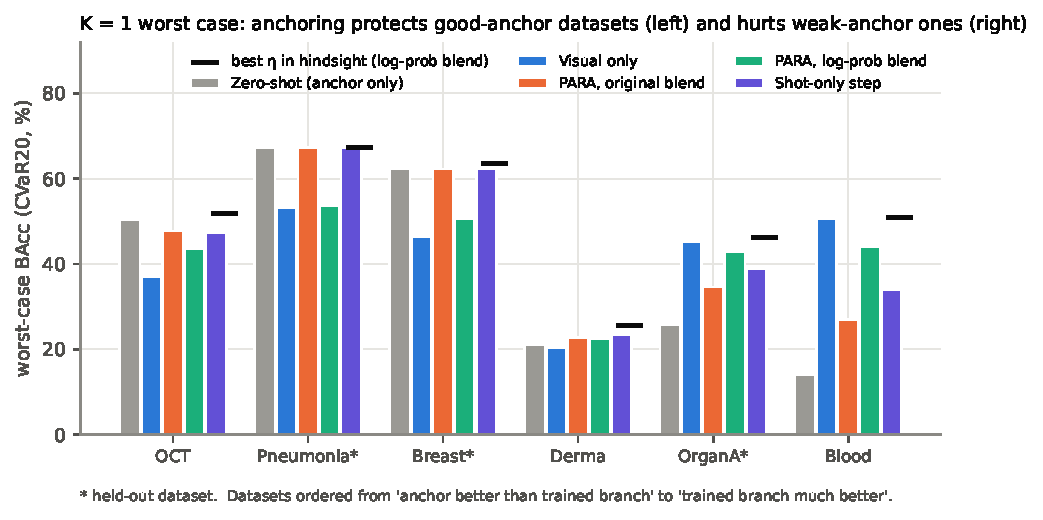
\includegraphics[width=\linewidth]{F5_worst_case_K1}
  \caption{Worst-case BAcc (CVaR20) at $K = 1$.
  The first three datasets are those where the anchor matches or beats the trained branch on mean BAcc at $K = 1$,
  the last three those where the trained branch is better. Held-out datasets are marked with an asterisk.
  The log-probability bars are discussed in Section~\ref{sec:finding4}.}
  \label{fig:worst_case}
\end{figure}

\paragraph{The best step follows relative anchor quality.}
The best step in hindsight (chosen on the test set) varies widely: from $0.17$ to $0.95$ for the log-probability blend of Section~\ref{sec:finding4},
and from $0.49$ to $0.98$ for the standardized blend on the multi-class datasets
(on binary datasets the standardized blend has no unique best step, Section~\ref{sec:finding2}).
It is ordered by the gap between zero-shot and visual-only BAcc (Figure~\ref{fig:best_eta}):
the Spearman correlation is $-0.80$ over all 18 (dataset, $K$) cells for the log-probability blend
and $-0.94$ over the 12 multi-class cells for the standardized blend (both $p < 0.001$).
This gap is computed on test labels, so it is a diagnostic of what the step should track, not a usable rule.
PARA's step, by contrast, is one value per $K$ (the dashed lines).

\begin{figure}[t]
  \centering
  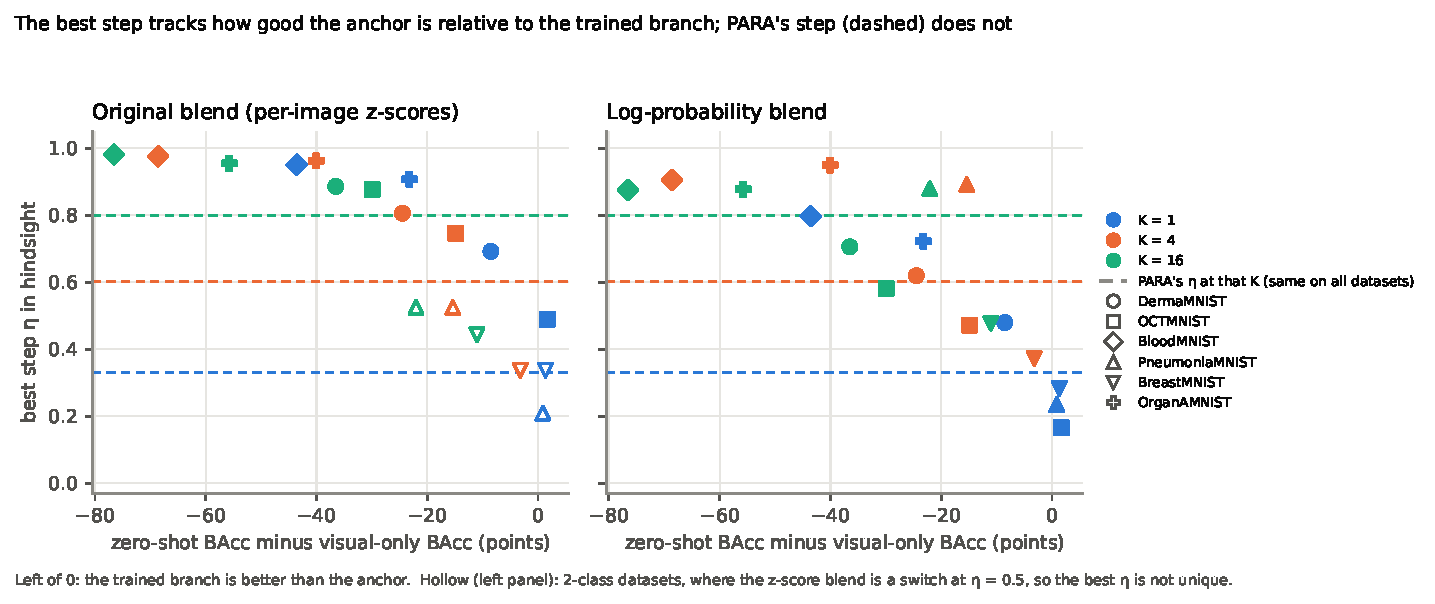
\includegraphics[width=\linewidth]{F4_best_eta_vs_relative_anchor}
  \caption{Best step in hindsight against zero-shot minus visual-only BAcc, one point per dataset and $K$,
  for the standardized blend (left) and the log-probability blend (right).
  Dashed lines: PARA's step at each $K$, which is the same on every dataset.
  Hollow markers (left): binary datasets, where the standardized blend is a switch and the best step is not unique.}
  \label{fig:best_eta}
\end{figure}

\paragraph{A rule fixed in advance: anchor reliability alone.}
A usable rule must estimate reliability from the support set.
The anchor's side is easy to measure, because the anchor is the frozen model:
$r_a$ is the anchor's mean probability for the true class on the support images, rescaled so that chance is $0$ and perfect is $1$.
On the design datasets $r_a$ tracks the best step well (Spearman $-0.71$ over 18 settings, $p < 0.001$).
We therefore fixed, before running any held-out dataset, an \emph{anchor-aware} step that treats the anchor as $k_0$ extra labelled examples:
\begin{equation}
  \eta_{\text{aa}} = \frac{K}{K + k_0}, \qquad k_0 = c\,\frac{r_a}{1 - r_a}, \qquad c = 8,
\end{equation}
so that a useless anchor ($r_a \approx 0$) gives $\eta_{\text{aa}} \approx 1$, and a reliable one keeps the step low until $K$ is large
(the choice of $c$ is described in Section~\ref{sec:setup}).

\paragraph{It worked in-sample and failed on held-out data.}
Table~\ref{tab:T4_preregistered_rule} reports the rule minus each baseline.
On the design datasets it beats PARA by $4.77$ BAcc points (significantly better in 10 of 18 settings, 7 after Holm's correction, worse in none)
and shot-only by $2.12$; choosing $c$ by leave-one-dataset-out instead gives a similar $4.94$ over PARA.
On the held-out datasets it is worse than every baseline:
$-0.68$ BAcc against PARA, $-1.50$ against shot-only and $-2.20$ against visual only,
and its worst case is worse still, with CVaR20 lower by $4.05$, $4.82$ and $1.89$ points.
Against visual only it is significantly worse in 3 of 12 settings (2 after Holm's correction) and better in none.

\begin{table}[t]
\centering
\small
\caption{Anchor-aware rule minus each baseline. Wilcoxon per setting over 10 draws; counts of settings significantly better/worse ($p<0.05$). ``Holm'' applies Holm's correction across the settings of each row. With 10 draws the smallest attainable two-sided Wilcoxon $p$ is $2/1024 \approx 0.002$, so a Holm-significant setting is one where nearly every draw moves the same way. LODO picks $c$ by mean BAcc on the other design datasets. Counts of draws won and lost are in the CSV.}
\label{tab:T4_preregistered_rule}
\begin{adjustbox}{max width=\linewidth}
\begin{tabular}{llrrllrllr}
\toprule
Setting & vs & $n$ & $\Delta$BAcc & sig. & Holm & $\Delta$F1 & sig. (F1) & Holm (F1) & $\Delta$CVaR20 \\
\midrule
Design, in-sample (frozen c=8) & PARA & 18 & 4.77 & 10/0 & 7/0 & 5.00 & 9/2 & 7/1 & 4.05 \\
Design, in-sample (frozen c=8) & Shot-only & 18 & 2.12 & 6/0 & 6/0 & 2.17 & 7/3 & 6/2 & 2.21 \\
Design, in-sample (frozen c=8) & Visual only & 18 & 0.23 & 2/1 & 0/0 & 0.00 & 3/1 & 1/0 & 1.84 \\
Design, leave-one-dataset-out & PARA & 18 & 4.94 & 10/0 & 6/0 & 5.51 & 9/3 & 6/1 & 3.23 \\
Design, leave-one-dataset-out & Shot-only & 18 & 2.29 & 6/0 & 6/0 & 2.67 & 6/4 & 6/2 & 1.39 \\
Design, leave-one-dataset-out & Visual only & 18 & 0.40 & 3/1 & 1/0 & 0.51 & 4/2 & 0/0 & 1.02 \\
Held-out (frozen c=8) & PARA & 12 & -0.68 & 1/1 & 1/0 & -0.26 & 3/1 & 1/0 & -4.05 \\
Held-out (frozen c=8) & Shot-only & 12 & -1.50 & 1/3 & 1/1 & -1.16 & 2/2 & 1/1 & -4.82 \\
Held-out (frozen c=8) & Visual only & 12 & -2.20 & 0/3 & 0/2 & -3.08 & 0/4 & 0/3 & -1.89 \\
\bottomrule
\end{tabular}
\end{adjustbox}
\end{table}


\paragraph{Why it failed.}
Each held-out dataset broke the rule in a different way, and all three point to the missing half of the comparison.
\begin{itemize}
  \item \emph{OrganAMNIST: a decent anchor, a much better trained branch.}
  Its anchor reliability ($r_a = 0.196$) is higher than OCTMNIST's ($0.164$), so the rule keeps the step low ($0.367$ at $K = 1$).
  But the trained branch is far ahead (visual only $48.97$ BAcc against $25.71$ for zero-shot), and the best step is $0.91$.
  The rule reaches $37.86$; visual only reaches $48.97$.
  Over all 21 multi-class settings, including OrganAMNIST, the correlation between $r_a$ and the best step drops to $-0.45$.
  \item \emph{PneumoniaMNIST at $K = 4$: the anchor is good, but not good enough.}
  Its high anchor reliability (mean $r_a = 0.392$) keeps the step below the binary switch point on 7 of 10 draws (mean step $0.415$),
  so on those draws the rule returns the anchor. It reaches $71.12$ BAcc, while the trained branch has already reached $82.75$.
  \item \emph{BreastMNIST at $K = 1$: an unstable estimate.}
  With one image per class, $r_a$ varies so much between draws that the step falls on either side of the switch point
  (above $0.5$ on 11 of 20 draws, mean $0.528$).
  The draws that switch to the trained branch include its worst ones:
  CVaR20 is $46.49$, the visual-only value, against $62.28$ for PARA, which always stayed with the anchor.
\end{itemize}
In each case the rule saw only the anchor's reliability, while the right step depends on the anchor relative to a trained branch it cannot see.
The trained branch's reliability is hard to estimate on the support set, because the branch is fitted to those same images;
a reliability estimated in the frozen space underestimates the trained branch, and the step we built from it was worse than PARA's
($54.73$ against $57.54$ mean BAcc on the design datasets; Appendix~B).

\paragraph{Measuring the trained branch directly.}
The HOSO-style step does measure the trained branch, by holding out one shot per class.
Where the support set is large enough it can be accurate: on OrganAMNIST it comes within $0.10$ and $0.16$ points of the oracle at $K = 4$ and $16$
($65.75$ against $65.85$, $81.46$ against $81.62$).
On the binary datasets, a single held-out image per class makes it noisy:
on PneumoniaMNIST at $K = 16$ it reaches $83.31$ BAcc against $89.40$ for PARA, and its worst case falls back to the anchor's $67.35$ against $87.22$.
It also needs an extra training run per draw and cannot be used at $K = 1$.
A cheap, reliable estimate of the trained branch's accuracy relative to the anchor is, in our view, the missing ingredient for an adaptive step.
